\documentclass[11pt]{article}
\usepackage{amsmath, amssymb, array}
\pagestyle{plain}

\textwidth=6.5in
\hoffset-1in
\textheight=9in
\voffset-1in

\usepackage{enumitem}
\usepackage{pgfplots}
\usepackage{graphicx}
\usepackage{lipsum}
\usepackage{stfloats}
\usepackage{multicol}
\usepackage{minipage-marginpar}
\usepackage{tikz}
\setlength{\columnsep}{1cm}
\usepackage{pinlabel} % for pin labels on figure


\newcommand{\abs}[1]{\left| #1 \right|}


\begin{document}


\noindent MATH 1113   \quad\quad\quad\quad\quad Worksheet \quad\quad\quad\quad\quad\   Name \underline{\phantom{alphabetsoupismyveryveryfavorite}}\\ 
\noindent Section 4.5 \\




\noindent \textbf{Instructions:}  Work together in groups of  3 or 4 to complete the following problems.\\

\begin{enumerate}

\item Determine the amplitude and period of the function.
\begin{enumerate}
\item $y=7\sin(2x)$\\[.5in]
\item $\displaystyle y=\frac{1}{7}\sin(2\pi x)$\\[.5in]
\item $\displaystyle y=-7\cos\Big(-\frac{2}{3}x\Big)$\\[.5in]
\end{enumerate}

\item Identify the phase shift and indicate whether the shift is to the left or to the right.
\begin{enumerate}
\item $\displaystyle \cos(x-\frac{\pi}{3})$\vfill
\item $\displaystyle \cos(2x+\frac{\pi}{3})$\vfill
\item $\displaystyle \sin(2\pi x -\frac{\pi}{8})$\vfill
\end{enumerate}


\newpage
\item Let $f(x)=2\cos(x+\pi)-1$.

\begin{enumerate}

\item Determine the period, amplitude, and phase shift of $f(x)=2\cos(x+\pi)-1$.\vfill
\item Find an interval containing exactly one cycle (period).\vfill
\item Determine the $x$-values of the five key points in the cycle above.
$$x_1= \quad \quad \quad \quad x_2= \quad \quad \quad \quad x_3= \quad \quad \quad \quad x_4= \quad \quad \quad \quad x_5= \quad \quad \quad \quad$$
\vfill





\item Graph $f(x)=2\cos(x+\pi)-1$.

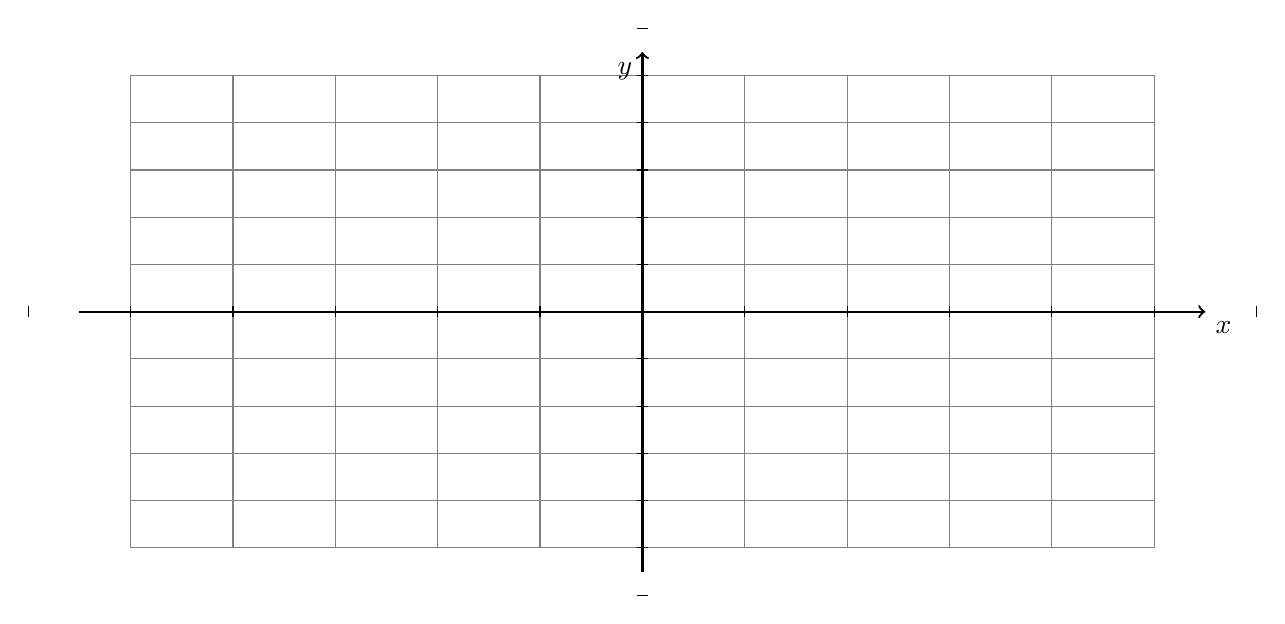
\begin{tikzpicture}[y=.6cm, x=1.3cm,font=\sffamily]
    %% ticks
    \draw[step = 1, gray] (-5,-5) grid (5,5);
    %% axis
    \draw[thick,->] (-5.5,0) -- coordinate (x axis mid) (5.5,0) node[anchor = north west] {$x$};
    \draw[thick,->] (0,-5.5) -- coordinate (y axis mid) (0,5.5) node[anchor = north east] {$y$};
    \foreach \y in {-6,-5,...,-1,1,2,...,6} {
      \draw (2pt, \y) -- (-2pt, \y);
    }
    \foreach \x in {-6,-5,...,-1,1,2,...,6} {
      \draw (\x,2pt) -- (\x,-2pt);
    }

  \end{tikzpicture}

\end{enumerate}


\newpage
\item Let $\displaystyle f(x)=-5\sin\Big(\frac{1}{3}x+\frac{\pi}{6}\Big)$.

\begin{enumerate}

\item Determine the period, amplitude, and phase shift of $\displaystyle f(x)=-5\sin\Big(\frac{1}{3}x+\frac{\pi}{6}\Big)$.\vfill
\item Find an interval containing exactly one cycle (period).\vfill
\item Determine the $x$-values of the five key points in the cycle above.
$$x_1= \quad \quad \quad \quad x_2= \quad \quad \quad \quad x_3= \quad \quad \quad \quad x_4= \quad \quad \quad \quad x_5= \quad \quad \quad \quad$$
\vfill





\item Graph $\displaystyle f(x)=-5\sin\Big(\frac{1}{3}x+\frac{\pi}{6}\Big)$.

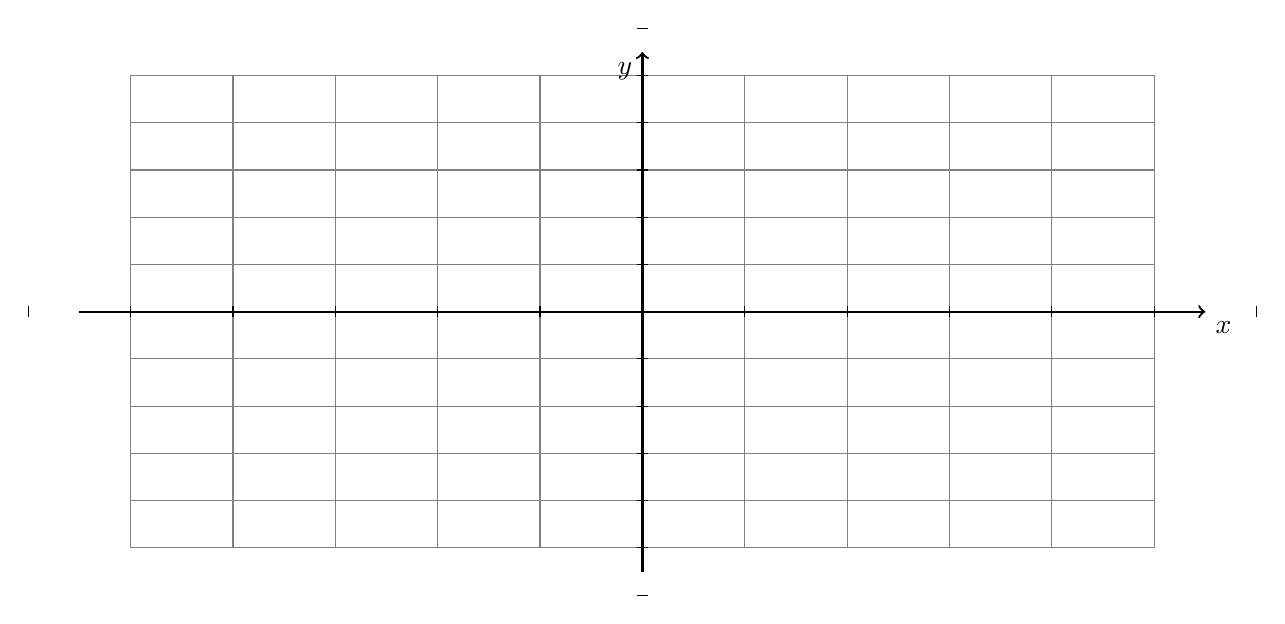
\begin{tikzpicture}[y=.6cm, x=1.3cm,font=\sffamily]
    %% ticks
    \draw[step = 1, gray] (-5,-5) grid (5,5);
    %% axis
    \draw[thick,->] (-5.5,0) -- coordinate (x axis mid) (5.5,0) node[anchor = north west] {$x$};
    \draw[thick,->] (0,-5.5) -- coordinate (y axis mid) (0,5.5) node[anchor = north east] {$y$};
    \foreach \y in {-6,-5,...,-1,1,2,...,6} {
      \draw (2pt, \y) -- (-2pt, \y);
    }
    \foreach \x in {-6,-5,...,-1,1,2,...,6} {
      \draw (\x,2pt) -- (\x,-2pt);
    }

  \end{tikzpicture}

\end{enumerate}


\newpage

\item Write an equation of the form $A\cos(Bx+C)+D$ for the given graph where $A>0$ and  $B>0$.

\begin{center}
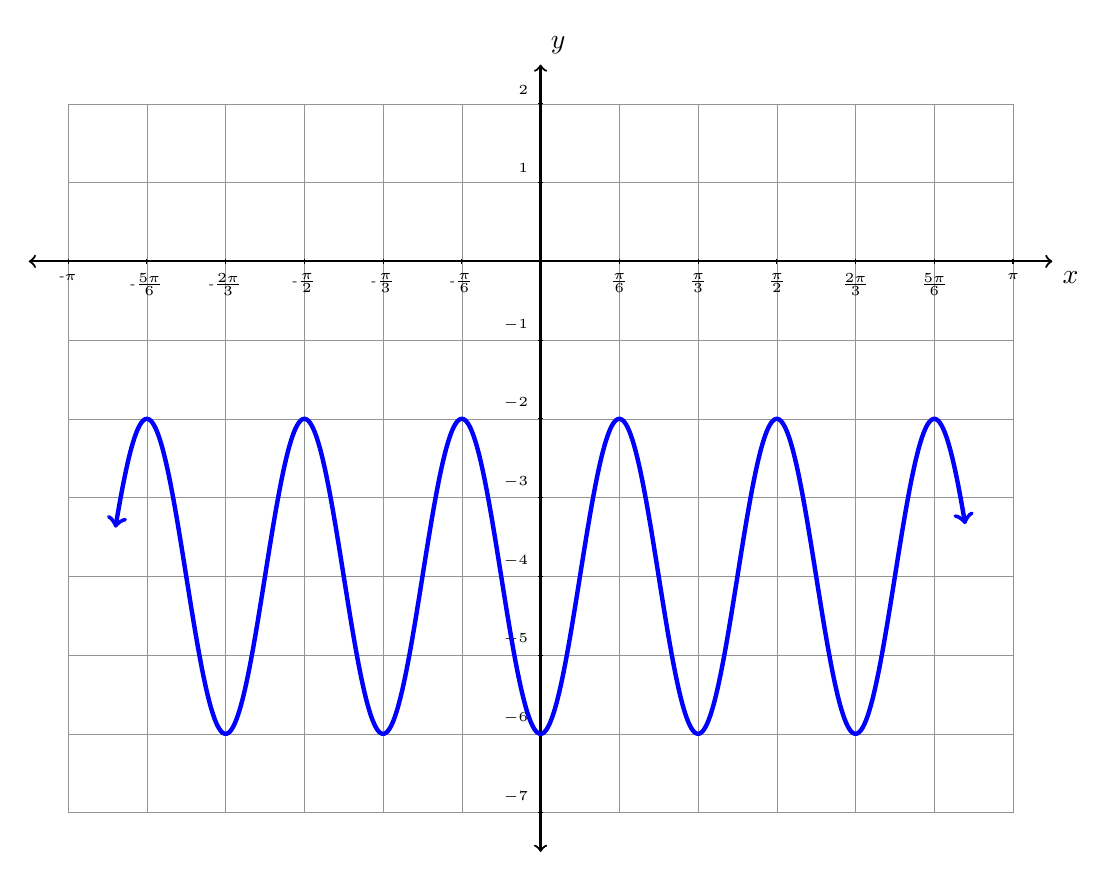
\begin{tikzpicture}[y=1cm, x=1cm,font=\sffamily,
	mydot/.style={
    circle,
    fill=white,
    draw,
    outer sep=0pt,
    inner sep=1.5pt
  }]
    %% Add a grid
    \draw[step = 1, gray, very thin,opacity=0.85] (-6, -7) grid (6, 2);
 	%% Draw the axes
	\draw[thick,<->] (-6.5,0) -- coordinate (x axis mid) (6.5,0) node[anchor = north west] {$x$};
    \draw[thick,<->] (0,-7.5) -- coordinate (y axis mid) (0,2.5) node[anchor = south west] {$y$};
    %% Label the y axis
    \foreach \y in {-7,...,-1,1,2,...,2} {
      \draw (1pt, \y) -- (-1pt, \y) node[anchor = south east] {\tiny $\y$};
    }
    %% Label the x axis
    %\foreach \x in {-5,...,-1,1,2,...,5} {
    %  \draw (\x,1pt) -- (\x,-1pt) node[anchor = north] {\tiny $\x$};
    %}
    \draw (-6,1pt) -- (-6,-1pt) node[anchor = north] {\tiny -$\pi$};
    \draw (-5,1pt) -- (-5,-1pt) node[anchor = north] {\tiny -$\frac{5\pi}{6}$};
    \draw (-4,1pt) -- (-4,-1pt) node[anchor = north] {\tiny -$\frac{2\pi}{3}$};
    \draw (-3,1pt) -- (-3,-1pt) node[anchor = north] {\tiny -$\frac{\pi}{2}$};
    \draw (-2,1pt) -- (-2,-1pt) node[anchor = north] {\tiny -$\frac{\pi}{3}$};
    \draw (-1,1pt) -- (-1,-1pt) node[anchor = north] {\tiny -$\frac{\pi}{6}$};
    \draw (1,1pt) -- (1,-1pt) node[anchor = north] {\tiny $\frac{\pi}{6}$};
    \draw (2,1pt) -- (2,-1pt) node[anchor = north] {\tiny $\frac{\pi}{3}$};
    \draw (3,1pt) -- (3,-1pt) node[anchor = north] {\tiny $\frac{\pi}{2}$};
    \draw (4,1pt) -- (4,-1pt) node[anchor = north] {\tiny $\frac{2\pi}{3}$};
    \draw (5,1pt) -- (5,-1pt) node[anchor = north] {\tiny $\frac{5\pi}{6}$};
    \draw (6,1pt) -- (6,-1pt) node[anchor = north] {\tiny $\pi$};

    %% Draw the function.
    \begin{scope}
%         \draw[very thick,blue] (-3,2) -- (1,1);
%         \draw[very thick,blue] (3.05,1.05) -- (4,3);
%         \draw[very thick,blue] (1.1,4) -- (3,4);
    %semi-circle
         %\draw[very thick, blue] (1,1) arc [radius=1, start angle=180, end angle= 5];
     %parabola
         %\draw[ultra thick, blue, domain=-5:0] plot (\x, {(-0.2)*(\x-5)*(\x+5)});
         \draw[ultra thick, blue, <->, domain=-5.4:5.4] plot[samples=1000] (\x, {-2*cos(pi*\x r)-4});             %dots
%         \fill[blue] (-3, 2) circle[radius=0.5ex];
%         \fill[blue] (1,1) circle[radius=0.5ex];
%         \fill[blue] (4,3) circle[radius=0.5ex];
%         \draw[very thick, blue] (3,1) circle[radius=0.5ex];
%         \fill[blue] (3,4) circle[radius=0.5ex];
%         \draw[very thick, blue] (1,4) circle[radius=0.5ex];


    \end{scope}

    %%\node[above=0.1cm] at (-2,2 )   {\nextXValue};

\end{tikzpicture}

\end{center}

\vfill


\newpage
\item Write an equation of the form $A\sin(Bx+C)+D$ for the given graph where $A>0$ and  $B>0$.

\begin{center}
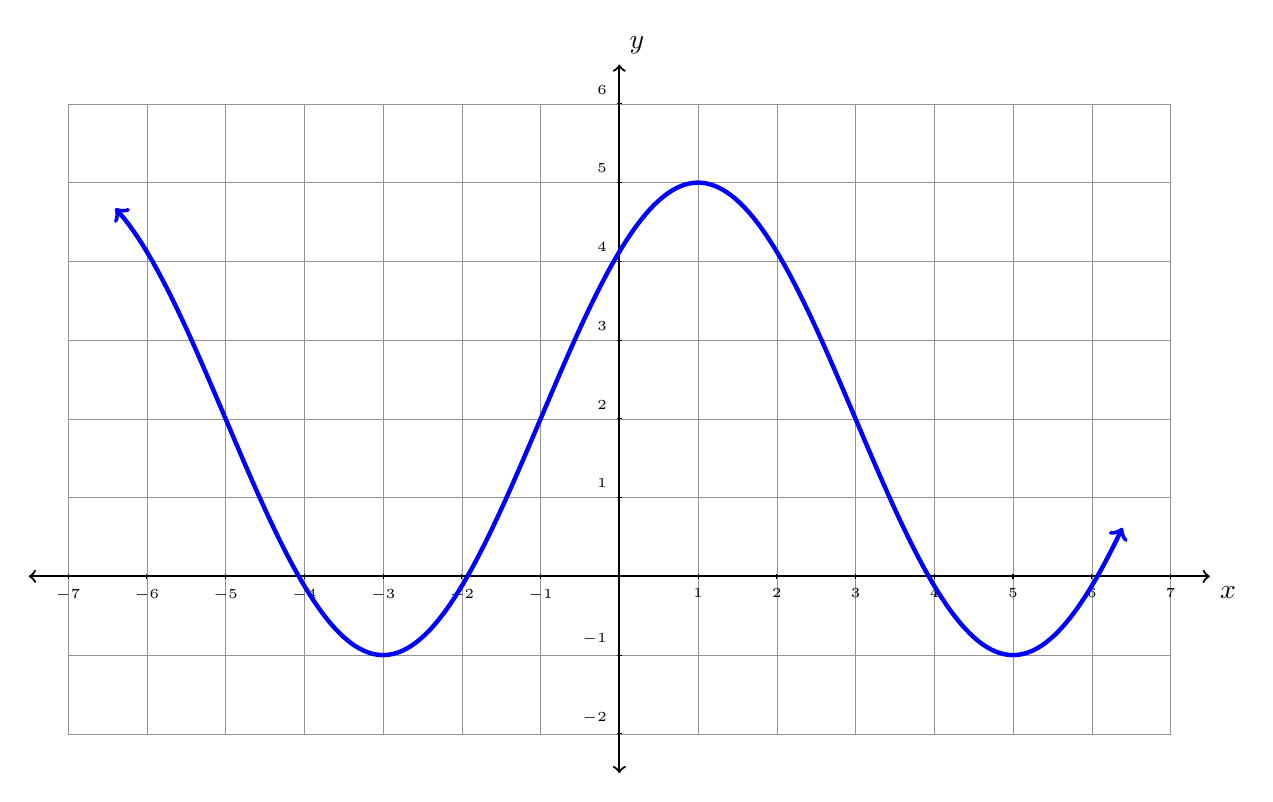
\begin{tikzpicture}[y=1cm, x=1cm,font=\sffamily,
	mydot/.style={
    circle,
    fill=white,
    draw,
    outer sep=0pt,
    inner sep=1.5pt
  }]
    %% Add a grid
    \draw[step = 1, gray, very thin,opacity=0.85] (-7, -2) grid (7, 6);
 	%% Draw the axes
	\draw[thick,<->] (-7.5,0) -- coordinate (x axis mid) (7.5,0) node[anchor = north west] {$x$};
    \draw[thick,<->] (0,-2.5) -- coordinate (y axis mid) (0,6.5) node[anchor = south west] {$y$};
    %% Label the y axis
    \foreach \y in {-2,...,-1,1,2,...,5,6} {
      \draw (1pt, \y) -- (-1pt, \y) node[anchor = south east] {\tiny $\y$};
    }
    %% Label the x axis
    \foreach \x in {-7,...,-1,1,2,...,7} {
      \draw (\x,1pt) -- (\x,-1pt) node[anchor = north] {\tiny $\x$};
    }
    %% Draw the function.
    \begin{scope}
%         \draw[very thick,blue] (-3,2) -- (1,1);
%         \draw[very thick,blue] (3.05,1.05) -- (4,3);
%         \draw[very thick,blue] (1.1,4) -- (3,4);
    %semi-circle
         %\draw[very thick, blue] (1,1) arc [radius=1, start angle=180, end angle= 5];
     %parabola
         %\draw[ultra thick, blue, domain=-5:0] plot (\x, {(-0.2)*(\x-5)*(\x+5)});
         \draw[ultra thick, blue, <->, domain=-6.4:6.4] plot[samples=1000] (\x, {3*sin(pi/4*(\x+1) r)+2});             %dots
%         \fill[blue] (-3, 2) circle[radius=0.5ex];
%         \fill[blue] (1,1) circle[radius=0.5ex];
%         \fill[blue] (4,3) circle[radius=0.5ex];
%         \draw[very thick, blue] (3,1) circle[radius=0.5ex];
%         \fill[blue] (3,4) circle[radius=0.5ex];
%         \draw[very thick, blue] (1,4) circle[radius=0.5ex];


    \end{scope}

    %%\node[above=0.1cm] at (-2,2 )   {\nextXValue};

\end{tikzpicture}

\end{center}


\vfill



\newpage
\item The water level relative to the top of a boat dock varies with the tides.  One particular day, low tide occurs at midnight and the water level is 7ft below the dock.  The first high tide of the day occurs at approximately 6:00 AM, and the water level is 3ft below the dock.  The next low tide occurs at noon and the water level is again 7ft below the dock.\\
Assuming that this pattern continues indefinitely and behaves like a cosine wave, write a function of the form $w(t)=A\cos(Bt+C)+D$.  The value $w(t)$ is the water level (in ft) relative to the top of the dock, $t$ hours after midnight.

\newpage

\item Write the range of the function in interval notation.
\begin{enumerate}
\item $y=\sin(x)$\\[0.2in]
\item $y=\cos(x)$\\[0.2in]
\item $y=8\cos(2x-\pi)+4$\vfill
\item $y=-3\cos(x+\frac{\pi}{3})-5$\vfill
\item $y=-6\sin(3x-\frac{\pi}{2})-2$\vfill
\end{enumerate}
\end{enumerate}

\end{document}